%\documentclass[aps,prd,nofootinbib]{revtex4-1}
\documentclass[singlepage,notitlepage,nofootinbib,11pt]{revtex4-1}
\usepackage{amsmath}
\usepackage{graphicx}
\usepackage{subfig}
\usepackage{epsfig}
\usepackage{listings}
\usepackage[hidelinks,hyperfootnotes=false,bookmarks=false,colorlinks=true]{hyperref}
\begin{document}
\title{Problem Set 2 - G6080}
\author{Victor Genty}
\email{vgenty@nevis.columbia.edu}
\homepage{www.nevis.columbia.edu/~vgenty}
%\affiliation{Department of Physics, Duke University, Durham, NC 27707, USA}
\date{\today}
\begin{abstract}
\centering
Source code can be found at \href{https://github.com/vgenty/G6080/tree/master/ps2}{github.com/vgenty/G6080/ps2}
\end{abstract}
\maketitle
\section{Problem 1 - Planets}
\subsection{Part 1}
\begin{figure}[h]
  \centering
  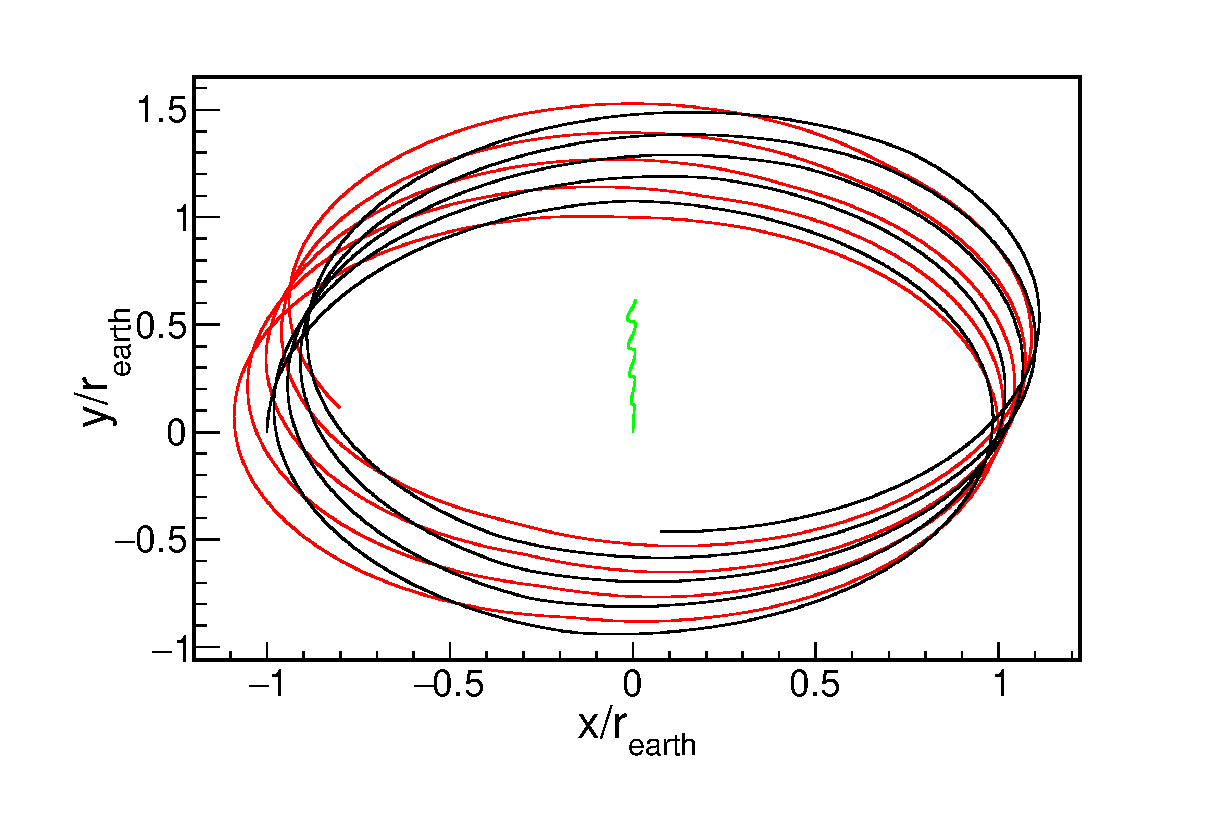
\includegraphics[width=0.5\textwidth]{figures/1r.eps}
  \subfloat[][]{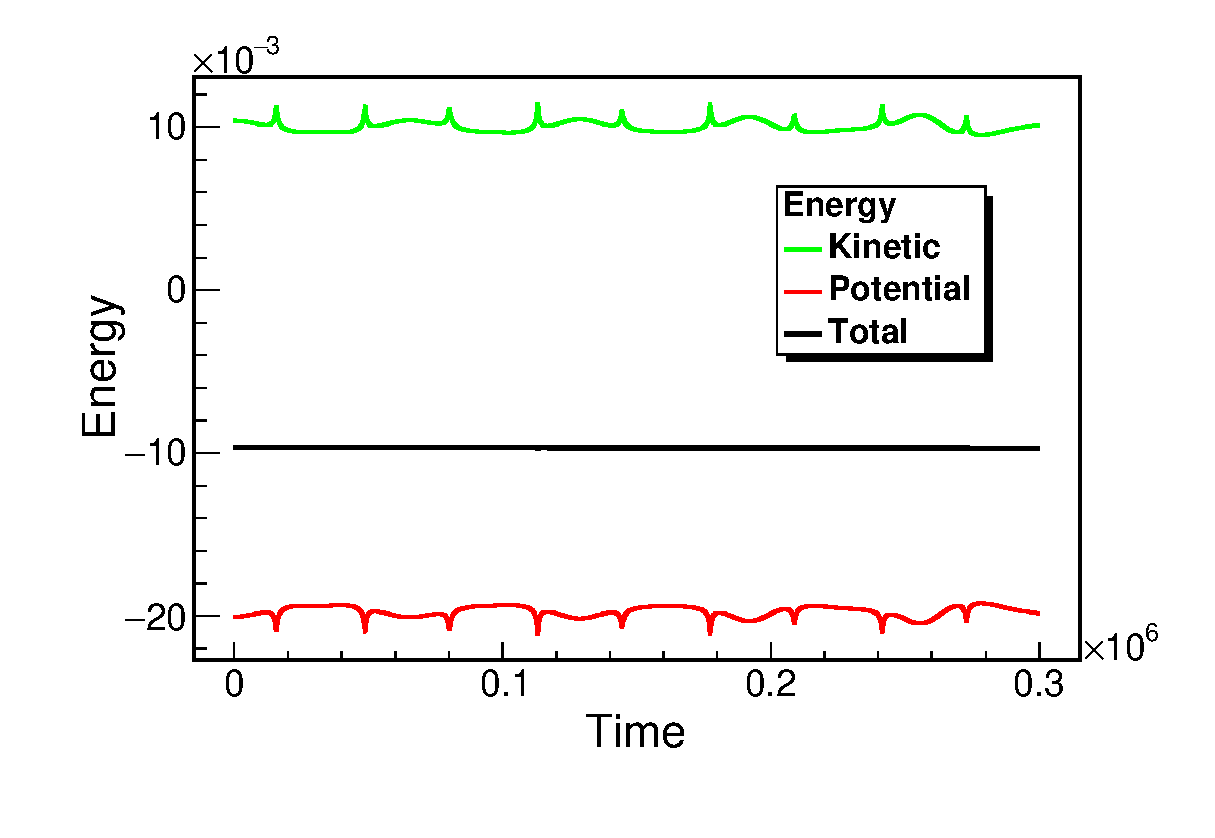
\includegraphics[width=0.5\textwidth]{figures/1es.eps}}
  \subfloat[][]{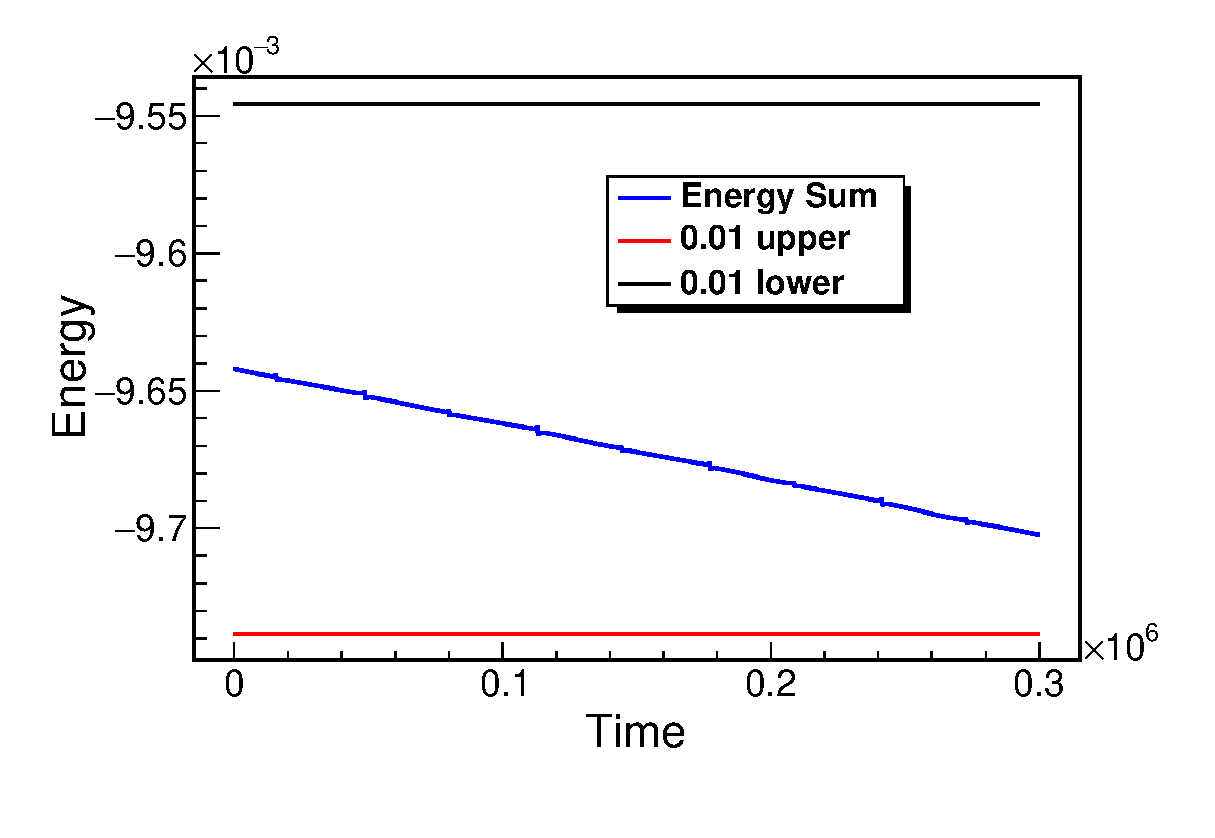
\includegraphics[width=0.5\textwidth]{figures/1ee.eps}}\\
\hfill
  \caption{Plots for Part 1. Top pane are the coordinate locations of the three planets the green, red, and black lines represent the trajectories of the sun and two orbiting planets. The bottom left pane shows the total kinetic and potential energies. The bottom right shows the deviation of the total energy as a function of time. The lines above and below represent 1\% bounds on the initial total energy.}
\end{figure}
\subsection{Part 2}
f
\subsection{Part 3}
d

\section{Problem 2 - LArgon}
\end{document}
